%% ----------------------------------------------------------------
%% Thesis.tex -- MAIN FILE (the one that you compile with LaTeX)
%% ----------------------------------------------------------------

% Set up the document
\documentclass[a4paper, 11pt, oneside]{Thesis}  % Use the "Thesis" style, based on the ECS Thesis style by Steve Gunn
\graphicspath{Figures/}  % Location of the graphics files (set up for graphics to be in PDF format)

% Include any extra LaTeX packages required
\usepackage[square, numbers, comma, sort&compress]{natbib}  % Use the "Natbib" style for the references in the Bibliography
\usepackage{verbatim}  % Needed for the "comment" environment to make LaTeX comments
\usepackage{vector}  % Allows "\bvec{}" and "\buvec{}" for "blackboard" style bold vectors in maths
\hypersetup{urlcolor=blue, colorlinks=false}  % Colours hyperlinks in blue, but this can be distracting if there are many links.
\usepackage{amsmath}
%% ----------------------------------------------------------------
\begin{document}
\mainmatter	  % Begin normal, numeric (1,2,3...) page numbering

% Set up the Title Page
\title  {Improving learning resource recommendations for students}
\authors  {\texorpdfstring
            {\href{CathalGeoghegan.me}{Cathal Geoghegan}}
            {Cathal Geoghegan}
            }
\addresses  {\groupname\\\deptname\\\univname}  % Do not change this here, instead these must be set in the "Thesis.cls" file, please look through it instead
\date       {\today}
\subject    {}
\keywords   {}

\maketitle
%% ----------------------------------------------------------------

\setstretch{1.3}  % It is better to have smaller font and larger line spacing than the other way round

% Define the page headers using the FancyHdr package and set up for one-sided printing
\fancyhead{}  % Clears all page headers and footers
\rhead{\thepage}  % Sets the right side header to show the page number
\lhead{}  % Clears the left side page header

\pagestyle{fancy}  % Finally, use the "fancy" page style to implement the FancyHdr headers

%% ----------------------------------------------------------------
% Declaration Page required for the Thesis, your institution may give you a different text to place here
\Declaration{

\addtocontents{toc}{\vspace{1em}}  % Add a gap in the Contents, for aesthetics

I hereby declare that this thesis is entirely my own work and that it has not been submitted as an exercise for a degree at any other university.
\bigskip
\bigskip
\bigskip
\bigskip
\bigskip
\bigskip
\bigskip


Signed:\\
\centerline{
    \rule[1em]{25em}{0.5pt}  % This prints a line for the signature
}
Date:\\
\centerline{
    \rule[1em]{25em}{0.5pt}  % This prints a line to write the date
}
}
\clearpage  % Declaration ended, now start a new page

%% ----------------------------------------------------------------
% The "Funny Quote Page"
%\pagestyle{empty}  % No headers or footers for the following pages

%\null\vfill
% Now comes the "Funny Quote", written in italics
%\textit{``Write a funny quote here.''}

%\begin{flushright}
%If the quote is taken from someone, their name goes here
%\end{flushright}

%\vfill\vfill\vfill\vfill\vfill\vfill\null
%\clearpage  % Funny Quote page ended, start a new page
%% ----------------------------------------------------------------

% The Abstract Page
\addtotoc{Abstract}  % Add the "Abstract" page entry to the Contents
\abstract{
\addtocontents{toc}{\vspace{1em}}  % Add a gap in the Contents, for aesthetics

In recent years there has been an explosion in the availability of educational resources.
One such kind of modern education resource have been Massive Open Online Courses such as Coursera.
With the widespread availability of education resources available there are challenges in finding the correct resources for students to use.
This project is to investigates the use of topic modeling and clustering algorithms to identify resources relevant to a topic in order to generate recommendations for students.

}

\clearpage  % Abstract ended, start a new page
%% ----------------------------------------------------------------

\setstretch{1.3}  % Reset the line-spacing to 1.3 for body text (if it has changed)

% The Acknowledgements page, for thanking everyone
\acknowledgements{
\addtocontents{toc}{\vspace{1em}}  % Add a gap in the Contents, for aesthetics

I would like to thank my father Peter and my mother Deirdre, who sadly passed away during this project.
They instilled in me a love for knowledge and education for which I will forever be grateful.
My friends Brendan, Emma, Darragh, Sam, and William for supporting me over the past four years.
The Computer Science society (DUCSS) in Trinity.
DUCSS without a doubt made the course ten times more enjoyable.
My supervisor Dr. Alexander O'Connor for his constant support and suggestions throughout this project.

}
\clearpage  % End of the Acknowledgements
%% ----------------------------------------------------------------

\pagestyle{fancy}  %The page style headers have been "empty" all this time, now use the "fancy" headers as defined before to bring them back


%% ----------------------------------------------------------------
\lhead{\emph{Contents}}  % Set the left side page header to "Contents"
\tableofcontents  % Write out the Table of Contents

%% ----------------------------------------------------------------
\lhead{\emph{List of Figures}}  % Set the left side page header to "List if Figures"
\listoffigures  % Write out the List of Figures

%% ----------------------------------------------------------------
\lhead{\emph{List of Tables}}  % Set the left side page header to "List of Tables"
\listoftables  % Write out the List of Tables

%% ----------------------------------------------------------------
%\setstretch{1.5}  % Set the line spacing to 1.5, this makes the following tables easier to read
%\clearpage  % Start a new page
%\lhead{\emph{Abbreviations}}  % Set the left side page header to "Abbreviations"
%\listofsymbols{ll}  % Include a list of Abbreviations (a table of two columns)
%{
% \textbf{Acronym} & \textbf{W}hat (it) \textbf{S}tands \textbf{F}or \\
%\textbf{LAH} & \textbf{L}ist \textbf{A}bbreviations \textbf{H}ere \\

%}
%% ----------------------------------------------------------------
% End of the pre-able, contents and lists of things

%% ----------------------------------------------------------------
\pagestyle{fancy}  % Return the page headers back to the "fancy" style

% Include the chapters of the thesis, as separate files
% Just uncomment the lines as you write the chapters
\lhead{\emph{}}  % Set the left side page header to ""
\chapter{Introduction}

\section{Introduction}

In this chapter I will give the motivation and the reasoning for the research carried out.
Following this, the research question is stated, the key objectives and challenges are examined and finally the outline of the report structure is laid out.

\section{Motivation}

Since ancient times, humankind has collated and archived the written knowledge of our species into collections.
From the Library of Alexandria to the modern day public library, humanity seems to have a need to preserve the knowledge of one generation to be presented to the next.
These collections have proved invaluable for students and scholars wishing to expand their own knowledge and understanding.

In recent years there has been a explosion in online learning resources.
From projects like the Internet Archive, Wikipedia, Project Gutenberg, and the rapid rise of the MOOC (Massive Open Online Course), we can see the human need to preserve and share knowledge continuing.
These systems, however, only provide the potential student with access to resources, they do not guarantee quality nor do they always facilitate a logical pathway to knowledge or understanding.

In the pre-digital age, some of the knowledge in these documents would have been catalogued by a human to make access easier.
The Dewey Decimal system used by libraries is an excellent example of the manual cataloguing of books to set topics.
However in the current digital age the flood of information is too huge to be finely catalogued by human operators.
There is also the problem of cataloging documents which could potentially contain a large number of varying topics.
This presents learners with the challenge of finding relevant information to suit their needs.

Often learners may be looking for information related to something they have already read, but are unable to bridge the gap between what they have already read, and what they should read next.
The aim of this project is to evaluate the use of popular machine learning algorithms to generate recommendations for a student.

More precisely this project will evaluate the performance of Latent Dirichlet Allocation, K-Nearest Neighbors, and Word2Vec.
The performance will be evaluated on temporal performance, quality of results and results compared to a gold standard.
Furthermore, this project will detail the background of each of the algorithms.

\section{Research Question}
The main research question that this project hopes to answer is; can we identify the best algorithm for resource recommendations by comparing their output on a varying corpus of academic papers?

\section{Objectives}
In order to answer the above research question there are three objectives we must first complete.

\begin{enumerate}
    \item Appropriate algorithms for generating recommendations must be first researched.
    From the algorithms researched, the most relevant today for generating recommendations must be chosen.

    \item A corpus must be selected that is relatively large and must contain a variety of topics.
    The corpus should also contain educational documents.

    \item The algorithms being evaluated are unsupervised and thus have no ideal model to compare against.
    To identify the best algorithm to use, an appropriate performance criteria must be decided on.

    \item Once the above objectives have been completed the algorithms chosen must be applied to the selected corpus.
    An evaluation of the performance of each of the algorithms must then be conducted.
\end{enumerate}

\section{Challenges}
As well as the objectives outlined above there are a number of challenges that must overcome before the research question can be answered.

\begin{enumerate}
    \item The selection of an appropriate educational corpus poses a problem due to the closed nature of publishing.
    Access to many academic papers and journals are often restricted to subscribers or members of professional organisations.

    \item The corpus selected must be a respected academic resource.
    As the research project is investigating the generation of recommendations in an educational context, the quality of the corpus should be to a high standard.

    \item Any algorithms or libraries chosen for the project will have differences which will have to be overcome.
    These differences could vary from function API's to how data is represented internally.

    \item The algorithms being investigated are unsupervised.
    This means that there is not a gold standard or previous model to compare the results to.
    The evaluation of the generated recommendations is therefore difficult, as it is largely subjective.
\end{enumerate}

\section{Thesis Outline}
Chapter 2 gives an analysis of machine learning and a detailed account of the current state of the art in content filtering.
This chapter will finish with a review of previous research in this field and how this project relates to that work.

Chapter 3 will describe the approach taken towards the problems, and the various design decisions that were made throughout the project.
This chapter will contain a breakdown of the project design as well as diagrams of the system architecture.

Chapter 4 will be an evaluation of the system design presented in Chapter 3.
Best practices and challenges encountered will be discussed in this chapter.
An unbiased evaluation of the system will also be made.

Chapter 5 will be an evaluation of the experiment results and a measure of the system's performance.
The criteria for a good learning resource will also be presented as well as any non-functional requirements.
A discussion of each of the algorithms chosen will also be presented individually and as a group.

Chapter 6 will conclude the report with a review of the project and results obtained.
A short overview of future work and how the system designed could be improved will also be presented.
 % Introduction

\chapter{}

In this section the background to the state of the art in machine learning and recomdation systems will be presented.
In particular the use of machine learning algorithms used as the content filtering component of recomendation systems will be discussed.
The different approaches to machine learning and recomendation systems will also be introduced and then discussed in detail.

\section{Background}
In 1947 Alan Turing presented a lecture to the London Mathematical Society in which he theorised that it would be possible for a machine to learn from it's experiences.
In Turing's example he proposed that learning be a prerequiste for a true intelligent system \cite{Turing1946}.
Turing further expanded on the concept of an intelligent machine in his 1950 paper which proposed a theorethical test, which he called the "imitation game", to identify whether machines could be considered intelligent \cite{Turing1950}.
This test has since become know as the Turing test.

Machine learning and recomendation systems can be viewed as semi-intelligent machines which try to learn from data fed into them.
These machines are replacements for human operators who would have had to classify data or suggest recomendation in the past.
One of main reasons machines are used instead of humans for this task is largely due to the volume of data available.
Another factor to consider is the quality of results obtained from the system.
For example humans can be biased by their opinion when presenting their results or findings.
A machine on the other hand generates it's results using the model it has created using the data that has been presented to it.
This approach is less likely to be skewed by personal bias when the model has been created using a balanced dataset\cite{FProvost2000}.

\section{Machine Learning}
Machine learning is an interdisiplinary field concerned with the study of self learning systems.
Machine learning has applications in fields such as; statistics, mathmathics, computer vision, game theory, information retrival, software engineering, sentiment analysis, artifical intelligence.

Machine learning algorithms try to build a model of a dataset by learning the patterns in the data.
The result of this is that machine learning algorithms can output seeminly intelligent results for data it has never seen before.

Machine learning can be split into three different types of learning:
\begin{itemize}
    \item Supervised learning
    \item Reinforced learning
    \item Unsupervised learning
\end{itemize}

\subsection{Supervised learning}
Supervised learning is a machine learning technique which tries to create a model which maps inputs to desired outputs.
This can be represented as a function f(x) which maps an input \(x_i\) to an output \(y_i\).
This is acheived by using a training set T = \((x_i, y_i)\) and a learning algorithm.
The learning algorithm produces a function \(\hat{f}(x_i)\) which can then be modified in response to the difference between \(y_i - \hat{f}(x_i)\).

\subsection{Reinforced learning}
Reinforced learning is a machine learning technique where the machine interacts with an environment and produces actions \(a_i\).
These set of actions interact with the environment which in turn results in the machine receiving rewards \(r_i\) from a rewards function.
The machine tries to learn how to create actions which maximises the future return on rewards.

\subsection{Unsupervised learning}
Unsupervised learning is a machine learning technique which tries to find hidden patterns in data.
An unsupervised learning algorithm receives inputs \(x_i\) but receives no desired outputs nor rewards.
The machine the tries to build a probalistic model of the data or it uses clustering to partion the data in categories.

The main difference between unsupervised techniques and other techniques is the lack of a clear measure of success.
This poises a problem when comparing the accuracy of different unsupervised techniques.
The effectivness of unsupervised techniques therefore rely heavily on heuristic approaches when judging their quality.

The research conducted in this project is focused on this type of machine learning.
Due to the fact that there is no gold standard to compare the quality of the similarity results, their effectiveness will be a matter of opinion.
Where possible the results will also be compared against any possible meta-data to help judge their effectivness.

\section{Recomendation Systems}
Recomendation systems are algorithms and technniques which try to generate recomenations for users.
The design of recomendation systems is an interdisiplinary field which touches upon information retrival, human computer interaction, machine learning, data mining, etc.
These systems often try to generate recomendations based on similarities between users or between content.
There are two main approaches used in recomendation systems;

\begin{itemize}
    \item Collaborative-filtering
    \item Content-filtering
\end{itemize}

\subsection{Collaborative-filtering}
Collaborative-filtering is an approach used by recomendation systems which tries to generate recomendations by comparing user data with other users.
The rationale behind this approach is to find similarities and differneces  between different groups of users and build a user model.
Once users have been grouped together recomendations can be generated based on what similar users have liked and disliked.
This type of recomendation system has been used extensively by Amazon when generating recomdations.

The main problem with this approach is that it requires a huge amount of inital data in order to generate appropriate recomendations.

\subsection{Content-filtering}
Content-filtering is an approach used by recomdation systems which learns to generate recomendations based on a users previous interations with an item.
This approach tries to learn the features of items in order to generate recomdations for items with similar features.

Unlike collaborative-filtering a huge amount of user data is not required for content-filtering.
The recomdations for this approach can be generated by building a model using the individual item features.

The research conducted in this project is focused entirely on the information filtering component of a content-filtering recomendation system.
The research project conducted was based on a potential user being a student.
However all of the algorithms investigated could be used in an content-filtering recomdation systems to filter recomendations based on the contenc of the items.

\section{State of the Art}
This research project is investigating the performance of LDA, k-NN and Word2Vec as the content-filtering component of a recomendation system.
Each of these algorithms have applications in information retrival and are not just confined to the field of recomendations systems nor an educational corpus.

\subsection{Latent Dirichlet Allocation}
LDA is a probalistic model for any discreate data but in this research project and most of the literature reviewed, textual data has been used.
LDA was introduced in 2004 by Blei, Ng and Jordan as an improvement on Deerwester's Latent Semantic Indexing (LSI) and on Hofmann's later Probalistic Latent Semantic Indexing (pLSI).
LDA was created in response to two problems identified with pLSI; the number of paramaters in the model grew linearly with the size of the corpus, and it was unclear as to how to assign a probability to a document that the model had never seen before.

LDA is hierarchical model which assumes that documents contain a mixture of topics and that topics are a mixture of word probabilities.
LDA is also a bag of words model which assumes that the topics are generated first and then documents are generated from these topics.
These assumptions are used when infering topics as it a reversing of the generation process.

LDA has been used in the past on a corpus of 17,000 articles from the magazine Science, with 100 topics.
The LDA model that was generated using this corpus was fed an unseen article on genome mapping and sequencing.
The distibution of topics in the article were then calculated and graphed.
It was found that the topics which seemed to be about; genetics, evoloution, disease, and computers had a high concentration in the article.

In a similar study to the above, LDA was applied to 21,434 articles from Science to create 50 topics.
The purpose of this experiment was to infer the most relevant topics from a document and then to find the most similar documents.

\subsection{k-NN}

\subsection{Word2Vec}

\section{Conclusion}
 % Background Theory

\chapter{Design}

\section{Introduction}
This chapter provides a description of the design decisions for the research project being conducted.
This builds upon the state of the art technology which was previously discussed in chapter 2.
In this chapter the requirements for the project are also discussed in relation to the objectives and challenges which were listed in chapter 1.
The overall system architecture will be presented in the form of UML diagrams.

\section{Requirements}
Based on the objectives and challenges as listed in chapter 1, the requirements can be split into corpus requirements and implementation requirements.
The corpus requirements deal with the selection of the corpus and sampling of the when test are run across different sizes of the corpus.
The implementation requirement deal with the three algorithms chosen and the different libraries used to implement them in the project.

\subsection{Corpus Selection}
In the context of generating recommendations for a student an academic or educational corpus should be used.
The availability of a large and respected educational corpus poises a problem however.
It was decided that academic papers from arXiv would act as a proxy for educational resources.
This in itself could create a problem due to how academic papers are usually written.
The language of an academic paper is usually quite different to the language used in a textbook or a lecture.
The language used is generally an advanced discussion of a particular subject, which itself could have it's own vocabulary.
This is particularly relevant for the arXiv corpus which has a large number of papers related to mathematics and physics.

While arXiv may not be the perfect educational corpus it is an adequate proxy.
The arXiv corpus could also be comparable to the corpus used by Blei in his paper on LDA.
In the Blei experiment, LDA was applied to approximately 22,000 articles from the journal Nature.
In that experiment Blei created an LDA model with 50 topics and used it to identify topics with documents and to find documents of a similar topic.

\subsection{Document Preprocessing}
The documents that are retrieved from the arXiv Amazon S3 bucket are saved as PDF documents.
As we are only interested in the textual content of the papers we must convert the PDF version of the papers to a plain text representation.
The size of the arXiv corpus was also considered during this step.
As each paper is independent of other papers, the conversion to plain text could be carried out in parallel.
This greatly speeded up the preprocessing stage as a four core machine could convert four papers at once.

Each of the arXiv papers follows the naming convention as follows: \textit{$\ll$topic-name$\gg\ll$paper-id$\gg$}.
This metadata can be used to sort the papers in directories based on their arXiv topic and to calculate the distribution of papers from specific areas.
More importantly this metadata allows us to compare the similar document recommendations generated against the arXiv topics.
If we consider the arXiv groupings to be a baseline we could assume that recommendations generated should return a large number of documents that are also in the same arXiv topic.

\subsection{Corpus Sampling}
The corpus selected contains approximately 50,000 academic papers from arXiv.
The corpus contains a mixture of papers from Physics, Mathematics, Computer Science and Nonlinear Sciences.
The papers are further split into smaller specific topics which have been selected by a moderator from arXiv.
There is however a disproportionate number of papers related to physics compared to the other sections.

As the algorithms are to be applied to a corpus of varying size the distribution of papers from each of the arXiv sections should be maintained.
This should be done in order to prevent papers from a particular topic or area from dominating the models generated.
If this was not done it would be possible that the algorithms could become too finely tuned to papers of a specific topic.
This could then result in the model generating a disproportionate number of recommendations from that particular topic.

To overcome this problem the system samples papers from each of the arXiv defined topics.
As different size corpus are tested a number of papers are randomly selected from each of the arXiv defined topics.
In order to ensure that the distribution of topics is consistent for every corpus size tested, the systems selects random papers so that the proportion of papers in each topic remains the same irrespective of corpus size.

\subsection{Algorithm Performance}
To adequately evaluate the performance of each of the algorithms the performance criteria has to be factored into the design of the system.
The performance criteria can be split into two main categories; temporal performance and the quality of similar document recommendations generated.

The temporal performance aspect of the project can be further split into two sections.
The time taken to build each of the models must be taken into consideration when evaluating the performance.
However the time taken to run similarity queries is also equally as important.
In a real world scenario it would be envisaged that the model would be built once or built as a batch job outside of peak times.
The similarity queries would probably not be run as batch jobs though due to the large number of documents which reside in the corpus.
Instead it would be envisaged that the similar document queries would be run as they are needed.
In this case the time taken to run queries should be relatively fast in order to have minimal effect on the user.

The quality of the recommendations generated are difficult to evaluate.
The algorithms used are all unsupervised and a gold standard to compare the results against is unavailable.
To try and overcome this problem two approaches could be use; the results generated could be compared against the arXiv topic metadata and a human could evaluate the quality of the recommendations generated by each of the models used.
Both of these approaches are not perfect but due to the size of the corpus and the nature of the algorithms used they will have to suffice.
Comparing against the arXiv metadata is imperfect as documents can contain multiple different topics.
The documents in arXiv however are catalogued into specific topic groupings which might not reflect the fact that the content of documents can be on the edge of different topics or areas.
Evaluating the quality of recommendations by hand is also imperfect due to the fact that it does not scale up well and depends on the person evaluating the recommendations to be able to spot the topic similarities between documents.

\subsection{Algorithm Tuning}

\section{System Archictecture}
\section{Conclusion}
 % Design

\chapter{Implementation}

In this chapter I explain the technologies used during the project and explain how the design laid down in chapter 3 was implemented.
Any challenges that were faced during the implementation are also discussed and contrasted with alternative approaches.

\section{Technologies}
Following an investigation of the field and the available technologies I decided that I would implement the system in Python.
Python is a dynamically typed language which has support for multiple different programming paradigms.
Python is widely used today both in industry and the scientific community.
Libraries such as NumPy, SciPy, matplotlib and pandas are widely used in the fields of data-analysis and scientific computing.
This has proven that Python is an adequate substitute for languages such as C, C++, Java, R, Matlab, etc.

Python also favors readability and minimalism compared to low level programming languages.
Despite being a relatively high level programming language, Python can also interface with C and C++ using the Cython library.
This is particularly useful when making code optimisations, such as vectorising code loops.

\subsection{Gensim}
Gensim is a Python toolkit for topic modeling and semantic analysis of textual data.
Gensim favours an online approach to training the models.
This achieved using Python generator expressions, which can result in only one document from the corpus residing in main memory at any one time.
This small memory footprint and incremental approach allows Gensim to scale in relation to the size of the corpus.
Gensim interfaces very well with NumPy and SciPy libraries.
As well as this it has been optimised to use the Cython library in order to speed up execution.

By using the Gensim toolkit I was able to gain access to the following tools:
\begin{itemize}
    \item build a dictionary of features from the corpus
    \item convert the corpus to a bag-of-words (bow) representation
    \item apply tf-idf transformations to bow models
    \item train LDA on bow models
    \item convert bow models to NumPy arrays
    \item train Miklov's Word2Vec model
    \item easily load and save different representations of the corpus
    \item use Gensim's native indexing for document similarities
\end{itemize}

As shown above Gensim is quite extensive in it's functionality and thus allowed me to manipulate the corpus easily.
This would have taken a considerable amount of time had I implemented all of this functionality myself.

\subsection{Annoy}
Annoy is a C++ library with Python bindings for approximate-Nearest-Neighbour search.
Annoy was created by Spotify to generate recommendations.
Within Spotify they use it find similar users and similar songs.
Spotify's system contains millions of tracks and has approximately 60 million active users.
This shows that Annoy is a tried and tested approximate-Nearest-Neighbour library which has scaled to large data-sets.

Annoy does approximate-Nearest-Neighbour queries by building an index using locality sensitive hashing (LSH) and random projections.
LSH is a technique used to reduce the dimensionality of high dimensional data by mapping them hash bins.
LSH tries to map similar items into the same bin and is very different to cryptographic functions which try to reduce the possibilities of collisions.
Random projections are dimensionality reduction technique which works by projecting the data into a random subspace of lower dimension.

Radim {\v R}eh{\r u}{\v r}ek, the creator of Gensim investigated the performance of different nearest neighbor libraries in November 2013.
In the final investigation the libraries were reduced down to just Annoy and FLANN.
During that investigation, Radim found that the query time for FLANN was approximately four times quicker than Annoy.
Annoy on the other hand had almost perfect accuracy (When compared to a non-approximate version of k-NN) compared to FLANN.

Annoy was selected for the k-NN investigation as:
\begin{itemize}
    \item Was found to be the most accurate approximate-Nearest-Neighbour library
    \item Easy to understand API
    \item Will be integrated into Gensim once the Boost library has been dropped as a requirement
    \item Has been shown to scale to very large data-sets
\end{itemize}

As shown above Annoy was chosen largely due to it's simplicity and the ease of integration with the Gensim toolkit.

\section{System Implementation}
In this section I outline the system that I built as prescribed in Chapter three.
Where possible UML has been used to describe the relations between the different components of the system.

\subsection{System}
\begin{figure}[h]
    \centering
        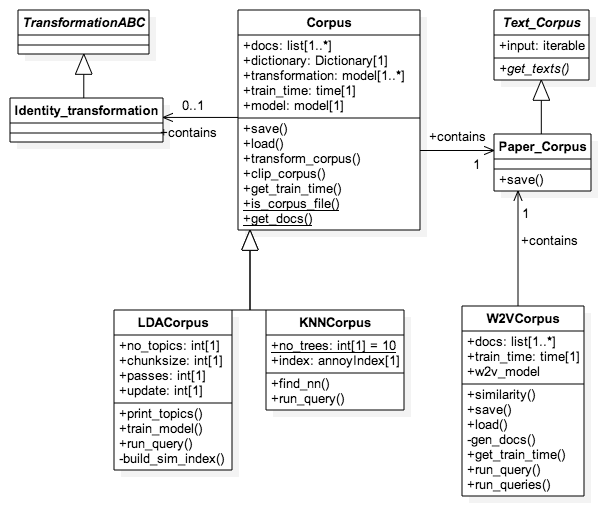
\includegraphics[width=0.7\textwidth]{Figures/FYPClassDiagram.png}
    \caption{System class diagram}
    \label{fig:UMLClass}
\end{figure}

Figure~\ref{fig:UMLClass} presents an overview of the system as a UML class diagram.
The main class in the system is the Corpus class.
The Corpus class is an abstract class used to represent a bag-of-words corpus.
The docs attribute is a list of document names from the corpus.
The dictionary attribute is a Gensim Dictionary object which represents the words in the corpus and their respective term frequencies.

The Corpus classes static function get\_docs is an interesting function used to generate a list of corpus files.
The function receives a path to a system directory, a dictionary of file distributions in sub-directories and a maximum number of files.
This function then generates a list of files from each of the sub-directory while maintaining the specified distributions.
The function then returns this flattened list of file paths.
This function is useful as it ensures that the same proportion of files will be sampled from each arXiv defined topic area, no matter the size of the corpus currently being tested.

The transformation attribute is used to represent transformation that have been applied to the bag-of-words corpus.
An interesting feature of Gensim is that you can stack corpus transformations on top of each other.
This for example could be used to apply a tf-idf transformation followed by an Latent-Semantic-Indexing transformation.
This however poised a small problem for the system.

When creating the above system, code readability and code reuse were huge factors that were considered.
In an earlier version of the project, if the corpus had a transformation applied, the transformation was only executed when iterating through the corpus.
However if a corpus did not have any transformations applied to it, this required an nested if-statement, which reduced code readability.

An alternative to this was to create an identity transformation which inherited from Gensim's TransformationABC class.
This Identity\_transformation is basically an identity function which returns the input document vector.
This approach was based on monad transformers from Haskell where the inner-most monad of stacked monad-transformers is either the identity monad or an IO action.
This eliminated the unnecessary conditional statement and increased the code readability by applying functional programming paradigms.

The Paper\_Corpus class is a wrapper around Gensim's Text\_Corpus class.
Gensim favours document streaming and is agnostic as to how the corpus is stored.
The corpus could be stored in one file or distributed across the web.
The Text\_Corpus is an abstract class which allows the user to use Pythons generator expressions to lazily load documents from the corpus and do any necessary pre-processing to the text.
As the arXiv corpus being investigated is organised as a collection of .txt files in multiple directories, this approach allowed the system to load documents one at a time and do some pre-processing to the text.
The pre-processing conducted includes; reading the document into memory, translating the text to lower-case, splitting the word-tokens on whitespace characters, and filtering out words that appear only once in the document.

Both the LDACorpus and the KNNCorpus files use a bag-of-words representation of the corpus and thus inherit from the Corpus class.
W2VCorpus on the other hand trains it's model using the plaintext corpus.
As stated above when implementing the system, code reuse and readability were two of the main factors considered.
When it came to implementing the Word2Vec model a choice was made to not inherit from the Corpus class even though there was some shared functionality.
This decision was made largely due to the difference in the semantics of the Word2Vec model and the models which used a bag-of-words representation.
This of course means that the DRY principle is violated but the shared functionality between the two classes is minor and separation ultimately increases the overall readability of the code.

The LDACorpus and the KNNCorpus are relatively small classes which inherit the majority of their functionality from the Corpus class.
The attributes for the LDA class and the k-NN expose the API for the underlying models imported from the Gensim and Annoy libraries.
Exposing the API allowed easier testing and tweaking of the algorithms being investigated.

\subsection{Code Harnesses}
Two code harnesses are used in the research project. The first harness is used to generate the LDA, k-NN and Word2Vec corpora and to log the time taken to generate each corpus.
The second harness is used to run similarity queries on each of the corpus files, log the time taken to run the similarity queries, log the results of each of the queries and then output the results in JSON.

\subsubsection{Generation Harness}
The generation harness is useful for the creation of corpora of varying size.
From the command line the script receives a list of corpus sizes to create, a corpus source directory and the algorithm to apply to the corpus.
An optional directory can also be passed as an argument to the script.
This optional directory is an output directory to store the generate corpus and model files.
If this directory is not specified a directory is created where the script is run and all files generated are stored in it instead.

The generation harness iterates through the list of corpus sizes and creates a corpus of that size.
For all of the algorithm apart from Word2Vec, a dictionary must be created and the corpus must be converted to a bag-of-words representation.
Word2Vec effectively skips this stage as it builds it's dictionary and model in the training stage.
For each corpus created, the time take to build the corpus is logged to a log file.
After the corpus and dictionary files have been created, the models is trained.
As Word2Vec differs from LDA and k-NN it trains using the original textual corpus.
LDA and k-NN on the other hand must use the dictionaries and bag-of-words representations created previously to train their models.
The times take to train each of the models is also logged to a file.

\subsubsection{Similarity Harness}
The similarity harness automates the process of using the models, which were generated by the generation harness, to query for similar documents.
The command line arguments for the similarity harness are very similar to the generation harness.
The script receives a list of corpus sizes, a directory of query files, a directory containing the previously generated models and the algorithm being tested.

For each of the sizes passed to the script, the list of query files is processed into the appropriate data representation.
For LDA and k-NN, the dictionaries created previously are loaded and the files from the query directory are converted to a bag-of-words representation.
For Word2Vec the process is slightly different because we need to find the word vector representations of the query documents before we can find similar documents.
This is achieved by loading the query documents and then adding them to the Word2Vec model.
This allows us to get a vector representation of the document which can be used to find similar words and similar documents.

The similarity queries are then run on each of the documents from the query corpus.
The time take to run the queries are logged to a file for later analysis.
The similar document results are also stored and later parsed to into readable JSON.
The similarity results are parsed into JSON in order to make them more portable.
This was done as there are some interesting Javascript libraries which could be used to visualise the results.

\section{Conclusion}
In this chapter the implementation of the system designed in chapter three has been described.
Any challenges encountered have been stated and their solutions explained.
In the following chapter, the results generated from the above system will be presented and analysed.
 % Implementation

\chapter{Evaluation}
In this chapter an outline the project findings is presented, using tables and graphs where appropriate.
An analysis of the corpus and the tests conducted to tweak the model parameters is presented.
The analysis of the temporal performance is then presented.
The temporal performance for building the models and the temporal performance for conducting document similarity queries will be presented.
The quality of the recommendations will then be analysed.
The quality will be evaluated using two criteria; comparison against the arXiv defined topic groupings and a manual evaluation of the document results.

\section{Corpus Analysis}
In this section an analysis of the arXiv corpus is presented.
The number of words or features present in the corpus are evaluated using a number of different filtering techniques.
The filtering technique used in the later evaluations will be compared against the other filtering techniques considered.

\subsection{Corpus Features}
The arXiv corpus consists to 50,400 documents from a number of arXiv topic groupings.
A breakdown of the groupings can be found in Table~\ref{table:arxivBreakdown}.
Approximately 30,000 of the papers are related to astrophysics, condensed matter and high energy physics.
The bias towards those topics may influence the models generated.
The removal of frequent and infrequent terms from the corpus will be presented.
An investigation was conducted to see if filtering out very frequent terms had a negative effect on the dictionaries generated.
As the aforementioned groupings make up approximately 60\% of the corpus, it was possible that filtering could remove words common to those papers.
As show in Table~\ref{table:frequentFeatures}, filtering out very common words had very little impact on the overall size of the corpus feature space.

\begin{table}[h]
    \centering
    \begin{tabular}{|c c|}
         \hline
         arXiv Topics & Number Documents \\ [0.5ex]
         \hline\hline
         astro-ph & 10572 \\
         cond-mat & 10262 \\
         hep-ph & 6770 \\
         hep-th & 5226 \\
         math & 4968 \\
         quant-ph & 2634 \\
         gr-qc & 2073 \\
         nucl-th & 1563 \\
         physics & 1511 \\
         hep-ex & 1257 \\
         nlin & 1120 \\
         math-ph & 815 \\
         hep-lat & 703 \\
         cs & 588 \\
         nucl-ex & 338 \\ [0.5ex]
         \hline\hline
         Total & 50400\\ [1ex]
         \hline
    \end{tabular}
    \caption{Breakdown of papers from arXiv topics}
    \label{table:arxivBreakdown}
\end{table}

Using all 50,000 arXiv documents with no filtering applied, there are 1,520,730 unique tokens in the corpus dictionary.
A large number of these features appear in only a small number of the documents (possibly noise caused by errors in the source document) or they appear in the majority of the documents.
Both of these can cause problems when creating the models.
A word that appears very few times in all of the documents is going to have very little impact on the quality of the models created.
This can lead to a very sparse feature space as each word vector will contain mostly zero entries.
By filtering out these infrequent terms it is possible to reduce the feature space and make the generated models more efficient by making the vectors less sparse. The following is an analysis of the size of the feature space as different filtering strategies were applied to the corpus.

\begin{figure}[h]
    \centering
        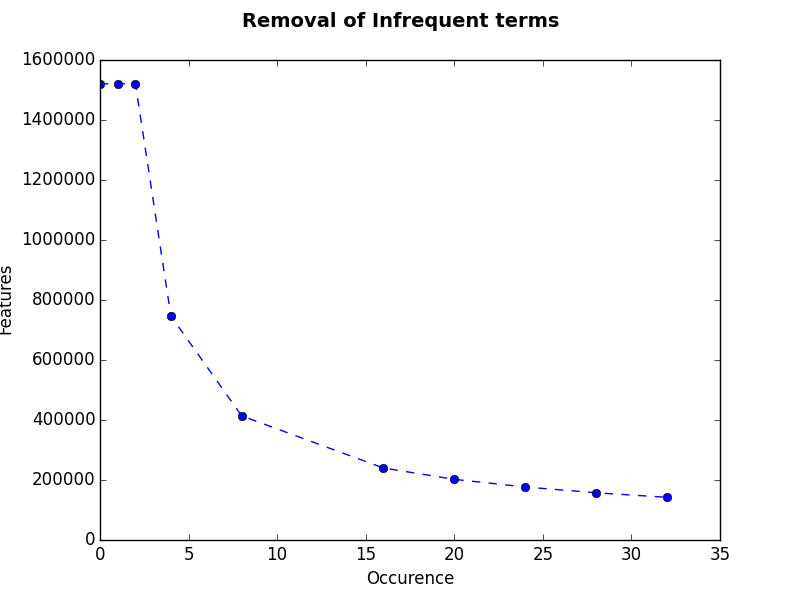
\includegraphics[width=0.7\textwidth]{Figures/CorpusFilterInfrequent.png}
    \caption{Feature space as infrequent words removed}
    \label{fig:FilterInfrequent}
\end{figure}

\begin{table}[h]
    \centering
    \begin{tabular}{|c c|}
         \hline
         Min Occurrences & Number Features \\ [0.5ex]
         \hline\hline
         0 & 1520730 \\
         1 & 1520730 \\
         2 & 1520730 \\
         4 & 746866 \\
         8 & 413733 \\
         16 & 239986 \\
         20 & 202237 \\
         24 & 176699 \\
         28 & 157388 \\
         32 & 142357 \\ [1ex]
         \hline
    \end{tabular}
    \caption{Number of feature as infrequent words filtered}
    \label{table:infrequentFeatures}
\end{table}

In Figure~\ref{fig:FilterInfrequent}, it can be seen that as infrequent words are filtered out, the size of the feature space shrinks dramatically until the filter amount reaches words that are in at least 20 documents.
The rate the corpus shrinks seems to level off at around 20-30 documents.
By filtering words using this strategy it was hoped that words which would be considered as noise would be removed from the dataset.

For each of the filtered dictionaries, a list of words whose frequency was one greater than the filter amount, was manually examined.
From the analysis of the sample features, a large number appeared to be random unicode characters, parts of mathematical equations, peoples names, or incomprehensible words.
An example of some of the words can be seen in Table ~\ref{table:infrequentWords}:

\begin{table}[h]
    \centering
    \begin{tabular}{|c c|}
         \hline
         Min Occurrences & Sample Words \\ [0.5ex]
         \hline\hline
         1 &  43+6, e−ih(tk, éri\\
         2 &  weiskopf9, 43+3, e−ih(t1\\
         4 &  (yt), nalysis, talbi\\
         8 &  82.70.-y, morsesmale, (1975\\
         16 &  ω(xf, 29.87, dnq\\
         20 &  5-ghz, 0.5-0.6, dolag\\
         24 &  δ(ei, (msd), pseudoclassical\\
         28 &  fic, thorlacius, ha3\\
         32 &  devriendt, hyung, fib\\ [1ex]
         \hline
    \end{tabular}
    \caption{Sample words removed from corpus}
    \label{table:infrequentWords}
\end{table}

\begin{figure}[h]
    \centering
        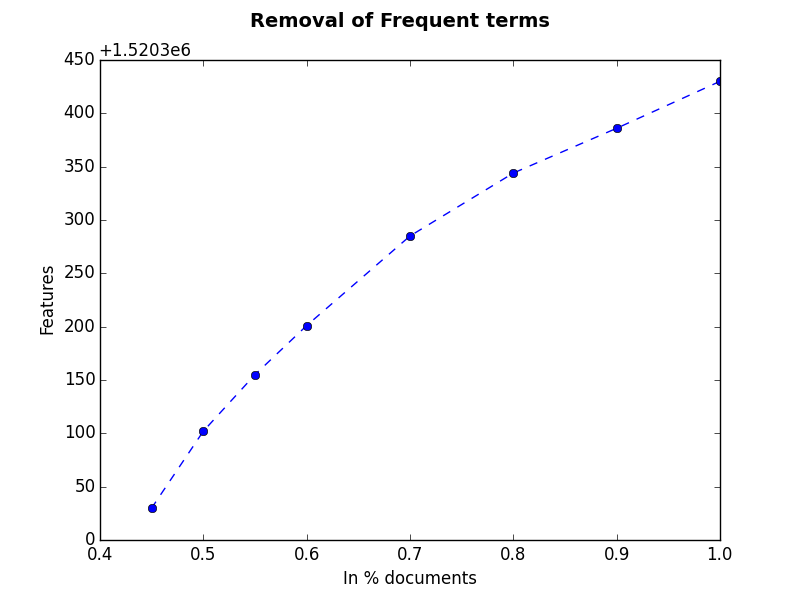
\includegraphics[width=0.7\textwidth]{Figures/CorpusFilterFrequent.png}
    \caption{Feature space as frequent words removed}
    \label{fig:FilterFrequent}
\end{figure}

\begin{table}[h]
    \centering
    \begin{tabular}{|c c|}
         \hline
         Percentage Occurrences & Number Features \\ [0.5ex]
         \hline\hline
         100 & 1520730 \\
         90 & 1520686 \\
         80 & 1520644 \\
         70 & 1520585 \\
         60 & 1520501 \\
         55 & 1520455 \\
         50 & 1520402 \\
         45 & 1520330 \\ [1ex]
         \hline
    \end{tabular}
    \caption{Number of feature as frequent words filtered}
    \label{table:frequentFeatures}
\end{table}

In Figure~\ref{fig:FilterFrequent} the effects of filtering out words which appear in a large percentage of the documents can be seen.
Compared to the filtering of infrequent terms shown previously, the filtering of frequent terms seems less effective.

These words are very likely to be words that would be very common English words such as "the", "and", "but", "a", "if", "or", etc.
These words are filtered from the corpus as they are so common in the documents that they are not distinguishable features that could be used to separate papers into different groupings.

From the above analysis of filtering the corpus, it was decided that terms that appeared in less than 20 of the documents or appeared in at least 75\% of the documents would be filtered out.
The lower bound of 20 was decided upon, as the number of features removed from the dictionary appeared to level off at around 20-25 minimum occurrences.
It was found that filtering out very frequent words had very little effect on the size of the dictionary.
The filter of 75\% was decided upon in order to remove very common words that could also have been removed using a list of stop-words.

\subsection{LDA Topic coherrency}
In this section the arXiv corpus was analysed by examining the quality of topics generated.
For this analysis, a sample of 3000 papers from the arXiv corpus was selected and the number of topics varied in multiples of 50 from 50-300.
The topics generated by the LDA algorithm were then manually evaluated.
This range was chosen based on the experiments conducted by Blei on the Nature corpus and a different corpus of arXiv documents\cite{BleiArXiv}.
It was found that generating models with 100 topics seemed to generate the most coherent topics.

Until version 0.11 of Gensim, the coherence of LDA topics was analysed by manually evaluating the topics generated.
In version 0.11 of Gensim, a function was added to sort topics based on their coherence.
This was based on the work of Mimno in his 2011 paper for evaluating the coherence of LDA topics\cite{Mimno}.
Unfortunately this update was released too late into the project to be used in the evaluation of LDA topics.
Future work into this research could use this functionality when choosing the number of LDA topics to use.

\section{Temporal Performance}
The temporal performance can be split into two sections; the time taken to build the models and the time take to run similarity queries on the models.

\subsection{Building Models}
The building of the models can be split into two stages;
the preprocessing of the corpus and then the training of the models.

Due to the differences in the three algorithms being evaluated, the time to preprocess the LDA and k-NN models will be naturally greater than Word2Vec.
This is due to the LDA and k-NN algorithms requiring a bag-of-words representation of the corpus.
First the corpus dictionary must be created by passing over the corpus once and the dictionary filtered of frequent or infrequent terms.
The corpus must then be passed over once more to translate each document into a bag-of-words representation.

Word2Vec, on the other hand, trains it's model on the textual representation of the corpus and doesn't require any extra pre-processing.
For this reason the time to preprocess LDA and k-NN is presented in Figure~\ref{fig:BuildBow}.

\begin{figure}[h]
    \centering
        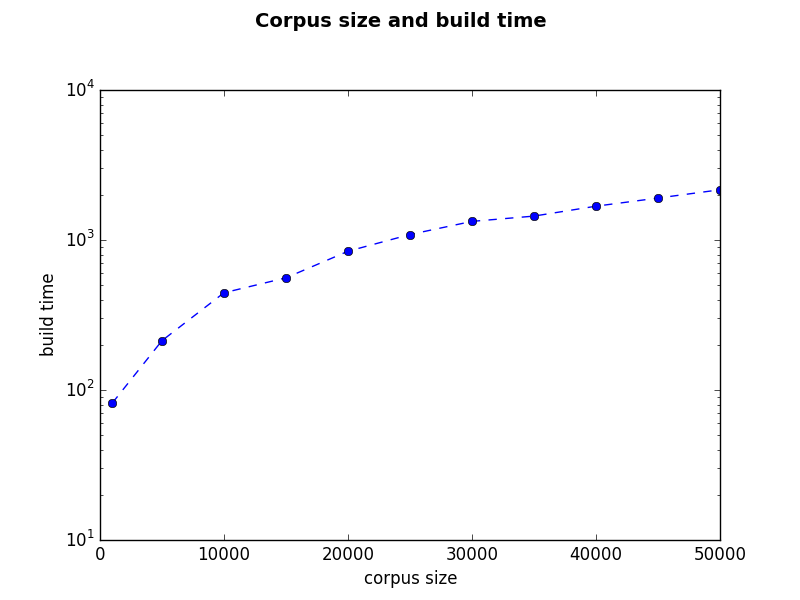
\includegraphics[width=0.7\textwidth]{Figures/BuildBOW.png}
    \caption{Time to preprocess LDA and k-NN}
    \label{fig:BuildBow}
\end{figure}

The time taken to train LDA, k-NN and Word2Vec is presented in Figure~\ref{fig:TrainAll}.
It should be noted that k-NN stops functioning at a corpus of approximately 35,000 documents.
This is due to the the underlying C++ library causing a segmentation fault as the size of the corpus increases.
This is possibly caused by the machine the models were being built on running out of memory.
When training a corpus of 30,000 documents it was noted that the process had allocate 21GB of virtual memory and was using approximately 90\% of physical memory.
K-NN's sudden spike at 30,000 documents is probably caused by thrashing as data is swapped from disc to physical memory.
The latency from reading from disc could account for the sudden increase in the train time.

\begin{figure}[h]
    \centering
        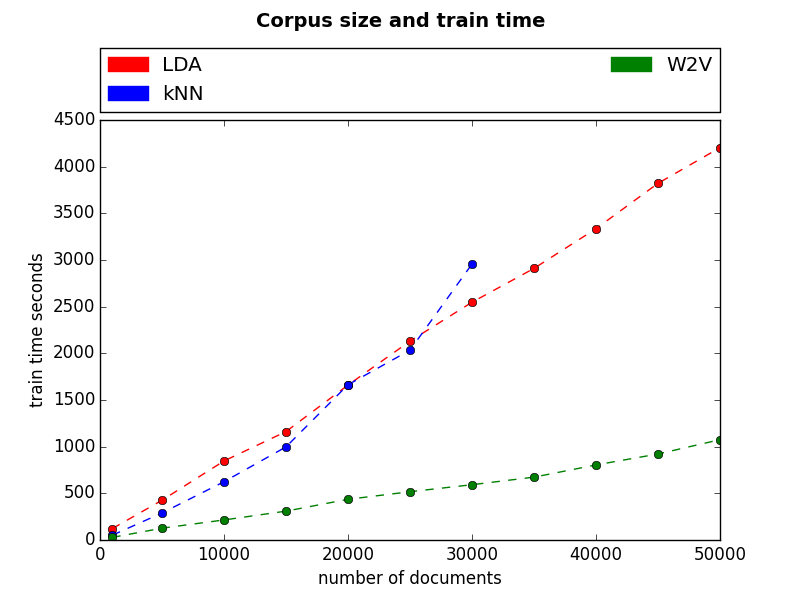
\includegraphics[width=0.7\textwidth]{Figures/TrainAll.png}
    \caption{Time to train LDA, k-NN, W2V}
    \label{fig:TrainAll}
\end{figure}

\subsection{Querying}
The querying of the recommendations was conducted by feeding 50 unseen documents into the models and logging the time taken to generate results.
The results generated from querying can be seen in Figure~\ref{fig:queryAll} and in Figure~\ref{fig:queryLDAKNN}.
As explained above, k-NN fails to create a model after approximately 30,000 documents.
This could also explain the high query time in relation to Word2Vec and LDA.
When k-NN is removed from the graph we can see that the query time of LDA remains almost constant, while Word2Vec grows as the size of the corpus grows.

\begin{figure}[h]
    \centering
        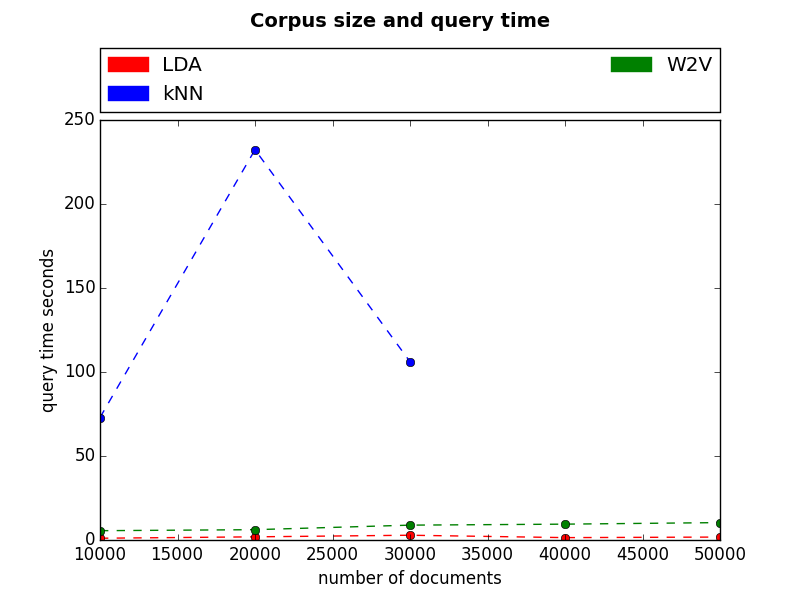
\includegraphics[width=0.7\textwidth]{Figures/queryAll.png}
    \caption{Time to query LDA, k-NN, W2V}
    \label{fig:queryAll}
\end{figure}

\begin{figure}[h]
    \centering
        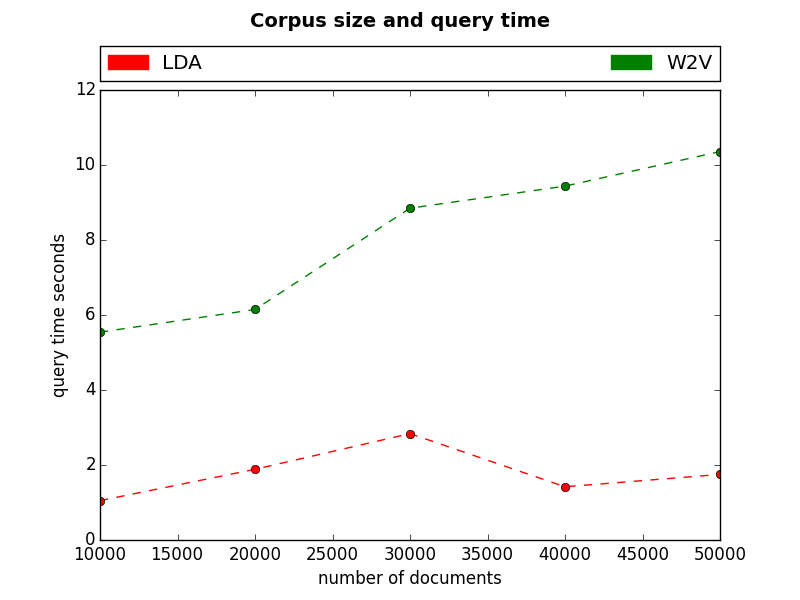
\includegraphics[width=0.7\textwidth]{Figures/queryLDAKNN.png}
    \caption{Time to query LDA, W2V}
    \label{fig:queryLDAKNN}
\end{figure}

\section{Recomendation Performance}
The recommendation performance of LDA, k-NN and Word2Vec is split into two sections.
For the manual analysis a sample of the recommendations are selected and evaluated based on their quality.
The arXiv comparison has been conducted by comparing the generated recommendations against the arXiv defined topics.

The query corpus consisted of 50 unseen documents, the breakdown of which can be found in Table~\ref{table:queryBreakdown}.
These queries were used on the models generated above.
However, unlike the above models which were generated on a corpus of ranging from 5,000-50,000 documents, the queries were applied to corpora increasing in size by 10,000 starting at 10,000 and finishing at 50,000 documents.

\begin{table}[h]
    \centering
    \begin{tabular}{|c c|}
         \hline
         arXiv Topics & Number Documents \\ [0.5ex]
         \hline\hline
         astro-ph & 10 \\
         cond-mat & 10 \\
         cs & 10 \\
         math & 10 \\
         physics & 10 \\ [0.5ex]
         \hline\hline
         Total & 50\\ [1ex]
         \hline
    \end{tabular}
    \caption{Breakdown of papers from query corpus}
    \label{table:queryBreakdown}
\end{table}

\subsection{Manual analysis}
As each of the algorithms being investigated are unsupervised and there is no gold standard to compare their results against, a manual evaluation of the results must be conducted.
This involved selecting three papers from each of the five arXiv topics and evaluating the quality of the recommendations generated.
In total 15 papers were selected and the top five recommendations generated by each of the algorithms were evaluated based on their coherence to the query document.
This process is prone to tedium and it is possible that the person classifying the documents may be unable to identify similarities due to a lack of knowledge in a particular field.

\subsection{arXiv comparison}
Unlike the manual comparison, which can only evaluate a small number of results, this comparison uses the arXiv meta-data to compare against the recommendations generated.
This is also imperfect due to the meta-data only associating each document with one topic when it could in fact be on the edge of two different topics.

An extensive breakdown of the arXiv results can be found in Appendix A.
Word2Vec seems to generate recommendations for papers which are in the arXiv topic for Mathematical Physics no matter what size the corpus is.
Surprisingly k-NN's recommendations are similar to the arXiv recommendations when the corpus is quite small.
As the size of the corpus grows, k-NN seems to generate recommendations from a small subsection of the arXiv topics.
Inversely, LDA seems to generate better results the larger the corpus becomes.
From this analysis it would seem that LDA is better at generating recommendations which are similar to the arXiv defined topics.

\section{Conclusion}
In this chapter the performance of LDA, k-NN and Word2Vec has been presented.
In temporal performance it was found that Word2Vec was the quickest at training a model of the corpus.
Word2Vec on the other hand generated very poor recommendations and would not be useful for this purpose.
The k-NN library used generated passible recommendations but it was not able to scale above 30,000 documents and may be unsuitable in a real world context.
The temporal performance of the LDA grew linearly with the size of the corpus and was comparable to k-NN until it failed.
LDA was also the quickest at generating recommendations for each corpus size examined.
The results generated by LDA also seemed to be the most coherent recommendations.

In the following chapter the conclusions from this research project will be presented and outline of any possible future work that could be conducted will be discussed.
 % Experiment and results

\chapter{Conclusion}
In this chapter there will be discussion of what this project achieved and how it addressed the research question as stated in chapter 1.
Any future work which could be done based on the work of this project will also be discussed.

\section{Summary}
The overall aim of this research project was to evaluated the performance of machine learning algorithms and pick the best one for generating document recommendations.

In chapter 1 the main objectives and challenges were outlined and briefly discussed.
During the course of this project: the state-of-the-art algorithms which could have been used were research, a large corpus of educational documents was sourced, the corpus was processed into the appropriate formats, models for each of the algorithms being evaluated were built, and an evaluation of the performance criteria as outlined in chapter 3 was conducted.

The temporal performance and quality of recommendations for LDA, k-NN and Word2Vec were evaluated and ranked on their overall performance.
It would seem that LDA was the best of the three algorithms for the corpus used.
LDA performed well for temporal performance and it consistently generated the best recommendations.
From this it can be concluded that of the 3 algorithms investigated, LDA is the better of the three if the intention is to generate document similarity recommendations.

\section{Future Work}
Further work should be carried out on this project to evaluate the performance of the machine learning algorithms.
Unfortunately only three algorithms were investigated but there are other machine learning algorithms which could have been used.
LDA is heavily influenced by LSI and pLSI and it would have been interesting to directly compare the performance of these algorithms alongside the ones investigated.

Another interesting piece of future work could be done to investigate the use of LDA and Word2Vec to summarise documents.
When presented with a document, LDA can be used to find the topic which has the highest influence on it.
As LDA's topics are constructed of word probabilities, they can be used to find words related to a document.
Word2Vec on the other hand can be used to find the words most similar to a given document.
Further work could be done to investigate the performance of LDA and Word2Vec for this type of categorisation.
 % Conclusion


%% ----------------------------------------------------------------
% Now begin the Appendices, including them as separate files

\addtocontents{toc}{\vspace{2em}} % Add a gap in the Contents, for aesthetics

\appendix % Cue to tell LaTeX that the following 'chapters' are Appendices

\chapter{An Appendix}
	% Appendix Title

%\input{Appendices/AppendixB} % Appendix Title

%\input{Appendices/AppendixC} % Appendix Title

\addtocontents{toc}{\vspace{2em}}  % Add a gap in the Contents, for aesthetics
\backmatter

%% ----------------------------------------------------------------
\label{Bibliography}
\lhead{\emph{Bibliography}}  % Change the left side page header to "Bibliography"
\bibliographystyle{unsrtnat}  % Use the "unsrtnat" BibTeX style for formatting the Bibliography
\bibliography{Bibliography}  % The references (bibliography) information are stored in the file named "Bibliography.bib"

\end{document}  % The End
%% ----------------------------------------------------------------
